\documentclass[a4paper]{tufte-handout}

\usepackage{amsmath}
\usepackage{amssymb}
\usepackage{amsthm}
\usepackage{bm}
\usepackage{authblk}
\usepackage{graphicx}
\usepackage{csquotes}
\usepackage{todonotes}
\usepackage{listings}

%% color and style from arXiv:1802.02538v1 source
\definecolor{codegreen}{rgb}{0,0.6,0}
\definecolor{codegray}{rgb}{0.5,0.5,0.5}
\definecolor{codepurple}{rgb}{0.58,0,0.82}
\definecolor{backcolour}{rgb}{0.99,0.99,0.97}
\lstdefinestyle{custom}{
  language=C++,
  literate={~}{$\sim$}{1},
  backgroundcolor=\color{backcolour},   
  commentstyle=\color{codegreen},
  otherkeywords = {real, vector, matrix, data, model, parameters, transformed},
  keywordstyle=\color{magenta},
  numberstyle=\tiny\color{codegray},
  stringstyle=\color{codepurple},
  emph={		normal, cauchy, inv_gamma, bernoulli_logit, gamma	},
  emphstyle=\color{codepurple},	basicstyle={\footnotesize,\ttfamily},
  breakatwhitespace=false,         
  breaklines=true,                 
  captionpos=t,                    
  keepspaces=true,                 
  numbers=left,                    
  numbersep=5pt,                  
  showspaces=false,                
  showstringspaces=false,
  showtabs=false,                  
  tabsize=2
}
\lstdefinestyle{customInline}{
  language=C++,
  literate={~}{$\sim$}{1},
  backgroundcolor=\color{backcolour},   
  commentstyle=\color{codegreen},
  otherkeywords = {real, vector, matrix, data, model, parameters, transformed},
  keywordstyle=\color{magenta},
  stringstyle=\color{codepurple},
  emph={		normal, cauchy, inv_gamma, bernoulli_logit, gamma	},
  emphstyle=\color{codepurple},	basicstyle={\ttfamily},
  breakatwhitespace=false,         
  keepspaces=true,                 
  numbers=left,                    
  numbersep=5pt,                  
  showspaces=false,                
  showstringspaces=false,
  showtabs=false,                  
  tabsize=2
}

\renewcommand{\v}[1]{\bm{#1}}
\newcommand{\vx}{\v{x}}
\newcommand{\vt}{\v{\theta}}
\newcommand{\vb}{\v{\beta}}
\newcommand{\vm}{\v{m}}
\newcommand{\R}{\mathbb{R}}
\newcommand{\E}{\mathbb{E}}
\newcommand{\Var}{\mathbb{V}ar}
\renewcommand{\P}{\mathbb{P}}
\newcommand{\Q}{\mathbb{Q}}
\newcommand{\D}{\mathcal{D}}

\newcommand{\eq}[1]{Eq.~(\ref{eq:#1})}
\newcommand{\fig}[1]{Fig.~\ref{fig:#1}}

\newtheorem{definition}{Definition}
\newtheorem{theorem}{Theorem}

%
% START COPYING HERE
%
\makeatletter
% Original definition of \cite from natbib package.
\DeclareRobustCommand\natcite{%
  \begingroup\let\NAT@ctype\z@\NAT@partrue\NAT@swatrue
    \@ifstar{\NAT@fulltrue\NAT@cites}{\NAT@fullfalse\NAT@cites}%
}

% Updated definition for Tufte-LaTeX
\renewcommand{\@tufte@infootnote@cite}[1]{%
  \natcite{#1}% <-- added this line
  \@tufte@add@citation{#1}%
}

% Only redefining this to get rid of a spurious space
\renewcommand\@tufte@add@citation[1]{\relax% adds a new bibkey to the list of cite keys
  \ifx\@tufte@citations\@empty\else
    \g@addto@macro\@tufte@citations{,}% separate by commas
  \fi
  \g@addto@macro\@tufte@citations{#1}% <-- stupid whitespace!
}
\makeatother
%
% STOP COPYING HERE
%

\renewcommand*{\thefootnote}{\fnsymbol{footnote}}

\title{Exploring COVID-19}

\author{Nils Bertschinger}
%% \author[1,2]{Nils Bertschinger}

%% \affil[1]{Frankfurt Institute for Advanced Studies, Frankfurt am Main, Germany}
%% \affil[2]{Goethe University, Frankfurt am Main, Germany}

\begin{document}

\maketitle%%

\renewcommand*{\thefootnote}{\Roman{footnote}}

\begin{abstract}
  The world stands still ... desperately observing the unfolding of
  the global COVID-19 pandemic.
\end{abstract}

\section{Data exploration}

The John Hopkins university and other institutes publish daily numbers
of cases and death tolls. Here, we build on their data sets and
provide some simple explorations and modeling.

\subsection{Country comparison}

\fig{rawdata} shows the raw data for several countries \footnote{Here,
  we only consider these countries in the following}.

\begin{figure}
  \begin{center}
    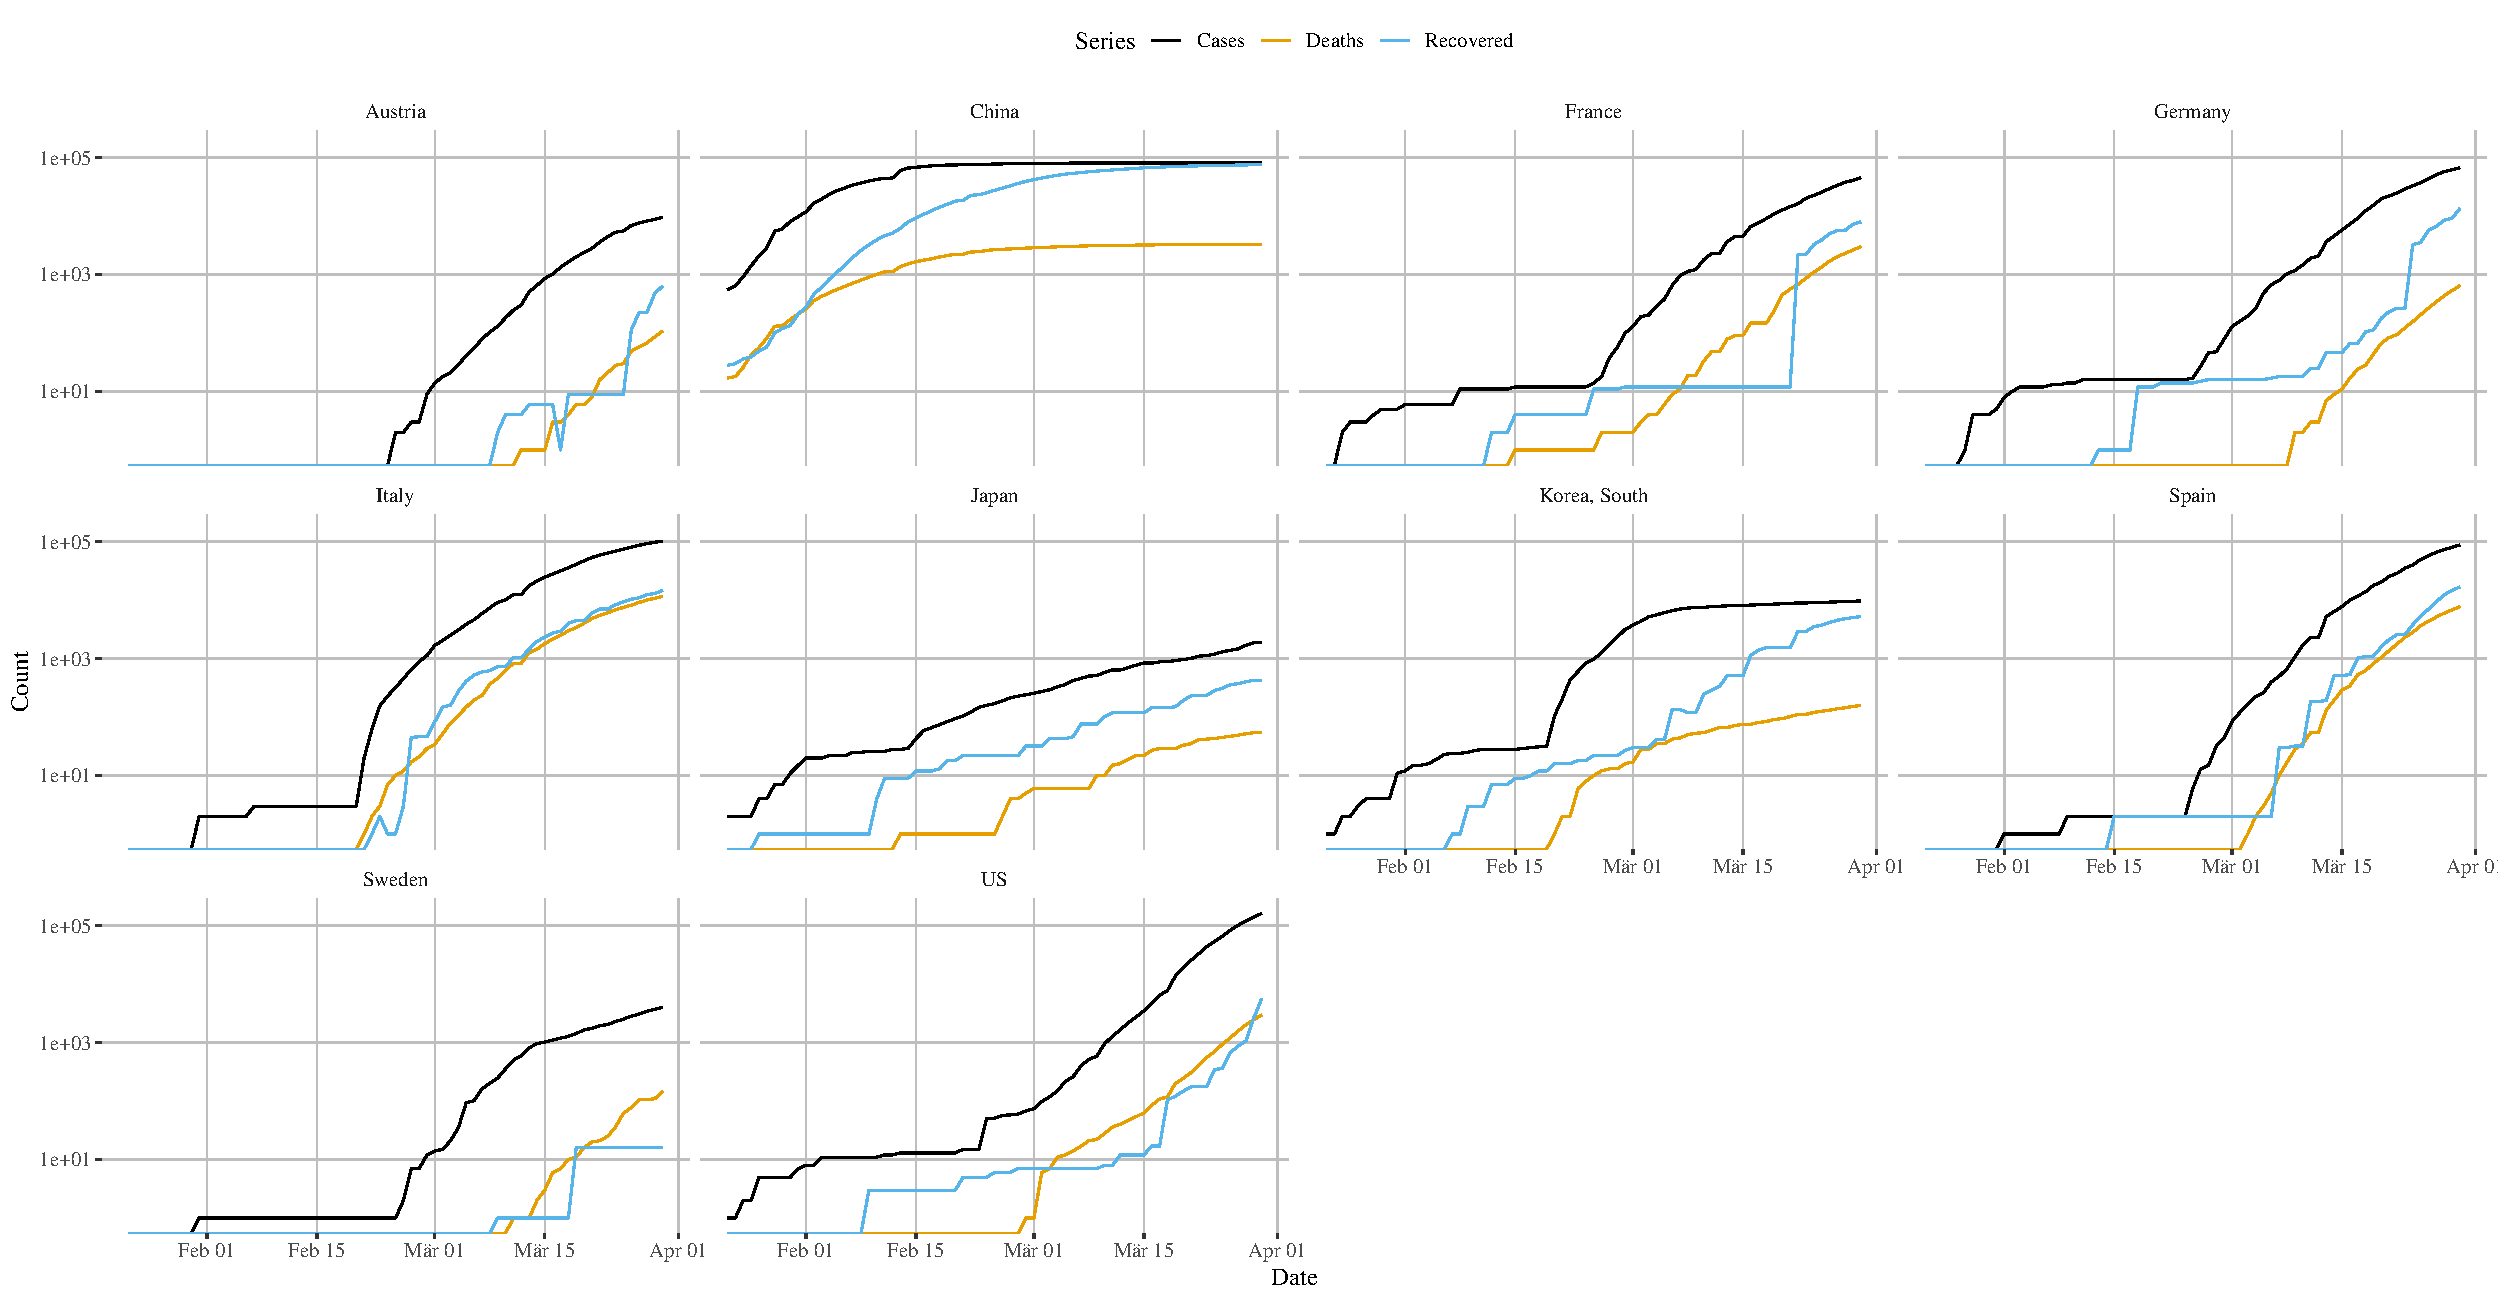
\includegraphics[width=0.95\textwidth]{../figs/raw_data.pdf}
  \end{center}
  \caption{\label{fig:rawdata}Data as provided by the John Hopkins
    university for some selected countries.}
\end{figure}

As the beginning of the epidemics is different in different countries
a direct comparison is difficult. Furthermore, especially the count of
cases is highly debated and plaqued with several uncertainties. Here,
we assume that the {\em death counts are reliable} and essentially
correct. Thus, in order to compare different countries we align all
curves such that day $0$ corresponds to the first day that the death
count reaches a specified threshold (either absolute or relative per
million inhabitants).

\begin{figure*}
  \begin{center}
    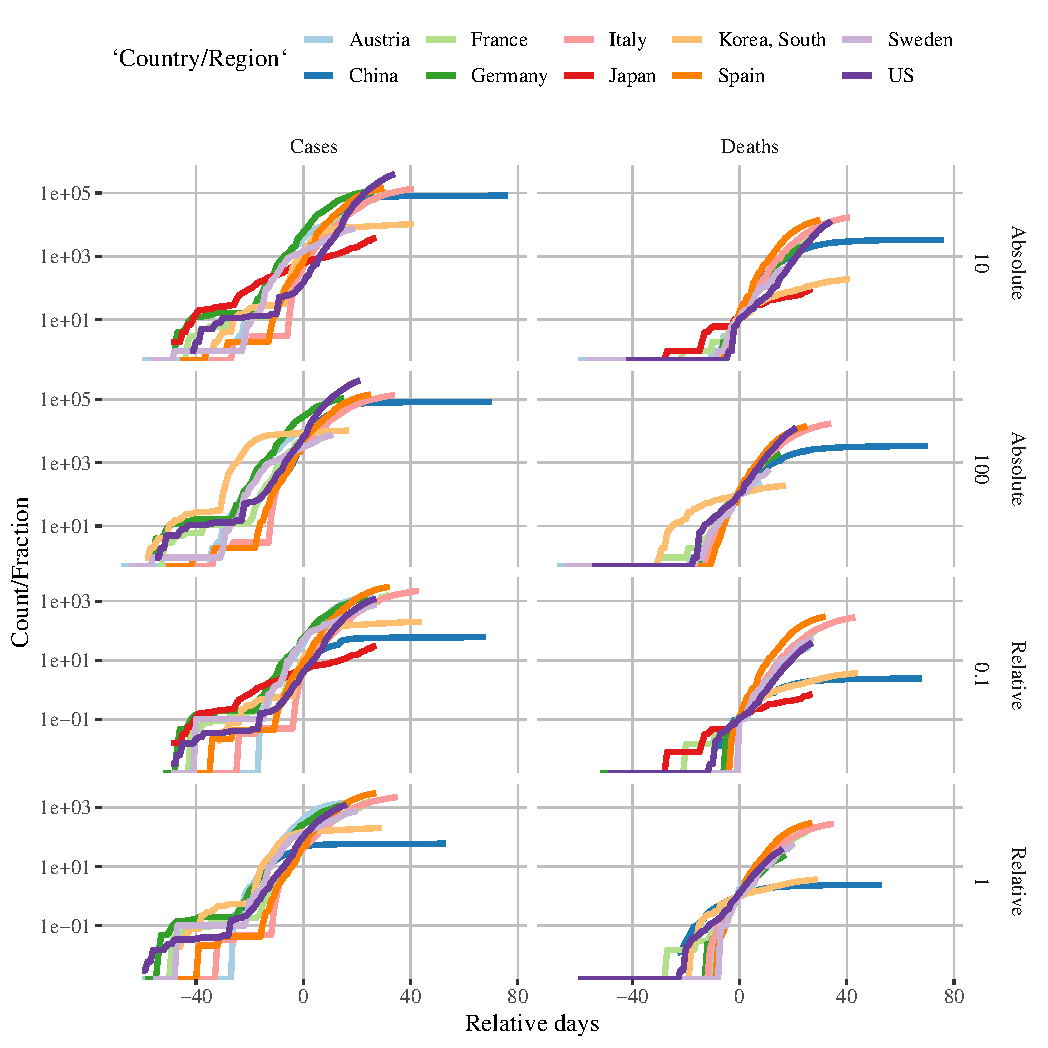
\includegraphics[width=0.95\textwidth]{../figs/align_data.pdf}
  \end{center}
  \caption{\label{fig:aligndata} Case and death counts aligned to
    first day of more than a specified threshold (either absolute or
    relative per million inhabitants).}
\end{figure*}

\fig{aligndata} shows a clear data collapse, especially at higher
thresholds\footnote{Note that some countries might not have reached
  these higher thresholds and are therefore not included in every
  subplot.} -- which are less noisy -- of 100 (absolute) or 1 per
million (relative). Furthermore, it is evident that the current growth
rate of China, South Korea (which are very similar in relative terms)
and Japan is markedly slower than of the other countries.

Interestingly, also the case counts are somewhat aligned even though
day zero has been defined purely based on the death
counts. Furthermore, there appear to be two groups of countries with
different systematic delays between case and death counts. In
particular, Austria and Germany seem to report deaths consistently
later than France, Italy and Spain. This suggests that the
surprisingly low death rate reported for Austria and Germany could be
an artefact as reported numbers are simply some days older compared to
other countries! This {\em delay effect} makes comparing numbers from
different countries difficult and also leads to unreliable estimates
when naively comparing numbers from same days only. Similarly, judging
the effectiveness of containment measures, e.g. social distances,
requires time as well within the second week after the intervention
has been established a majority of observed cases had probably been
infected already before the intervention.

\subsection{Statistical modeling}

\paragraph{Phenomenological growth model}
Overall, I believe it unlikely that the death rate is very different
across different countries\footnote{There are certainly demographic,
  medical or other aspects though.}. Next, I build a phenomenological
model on the assumption that the {\em death rate is constant across
  all countries} and differences purely arise from delays in reporting
positively tested cases and deaths. The model assumes the following:
\begin{itemize}
\item The probability of death is the same for all countries whereas
  the testing prevalence is country specific.
\item Observed counts are negative binomial distributed -- as an
  over-dispersed Poisson -- and delayed wrt the actual cases.
\item Actual case and death counts in each country grow according to a
  sigmoid function\footnote{A more realistic model should build on
    epidemic dynamics such as SEIR \ldots see below.} with country
  specific parameters\footnote{The basic model assumes \[ c(t) = a (1
    + e^{- \beta \nu (t - \tau)})^{- \frac{1}{\nu}} \; , \] i.e. a
    generalized logistic function.}.
\end{itemize}

As shown in \fig{taudie}, this model\footnote{Full code of this and
  other models can be found at my accompanying \href{Github}{\url{}}
  repository.} indeed finds a consistent difference in the delay of
death counts between Austria, Germany and France, Italy,
Spain. Furthermore, the death rate -- assumed constant across all
countries -- is estimated as $4.8 \pm {1.2 \atop 1.2} \%$. Estimates
in the range of 3 to 5\% appear to be rather robust for the present
model, yet seem to be somewhat too high\footnote{Note that a naive
  estimation of the death rate, i.e. dividing contemporal case by
  death counts is biased downwards by the delay effect as actual
  deaths only realize about a week later. Accordingly the death rate
  estimate should be based on the substantially lower case counts a
  week ago.}. It remains to be seen if my model estimate holds up over
time and wrt estimates derived from more realistic models \ldots

Detailed model predictions for all considered countries are shown in
\fig{modelpred}. The predictions are mostly reasonable, but the model
has difficulty of matching the rapid leveling off observed in China
and South Korea. Interestingly, the model predicts that the curve has
already slowed markedly in Germany and Italy even though this is
barely visible in the raw numbers by now -- another example of why the
delay effect is important in understanding the dynamics of the
COVID-19 pandemic. Yet, this model prediction relies heavily on the
assumption of sigmoidal growth and I would not be too optimistic about
it.

\begin{figure}
  \begin{center}
    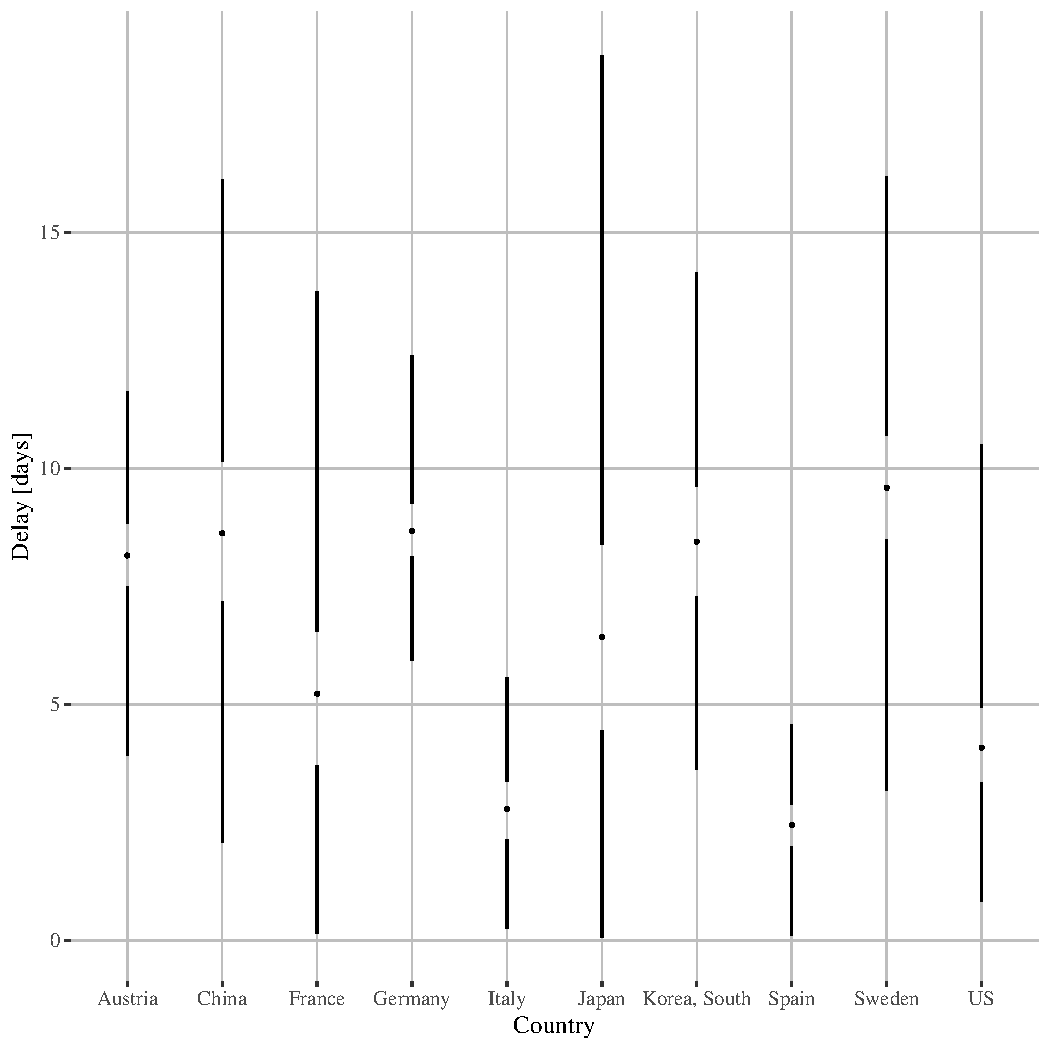
\includegraphics[width=0.95\textwidth]{../figs/tau_die.pdf}
  \end{center}
  \caption{\label{fig:taudie} Model estimated delay between reported
    case and death counts.}
\end{figure}

\begin{figure}
  \begin{center}
    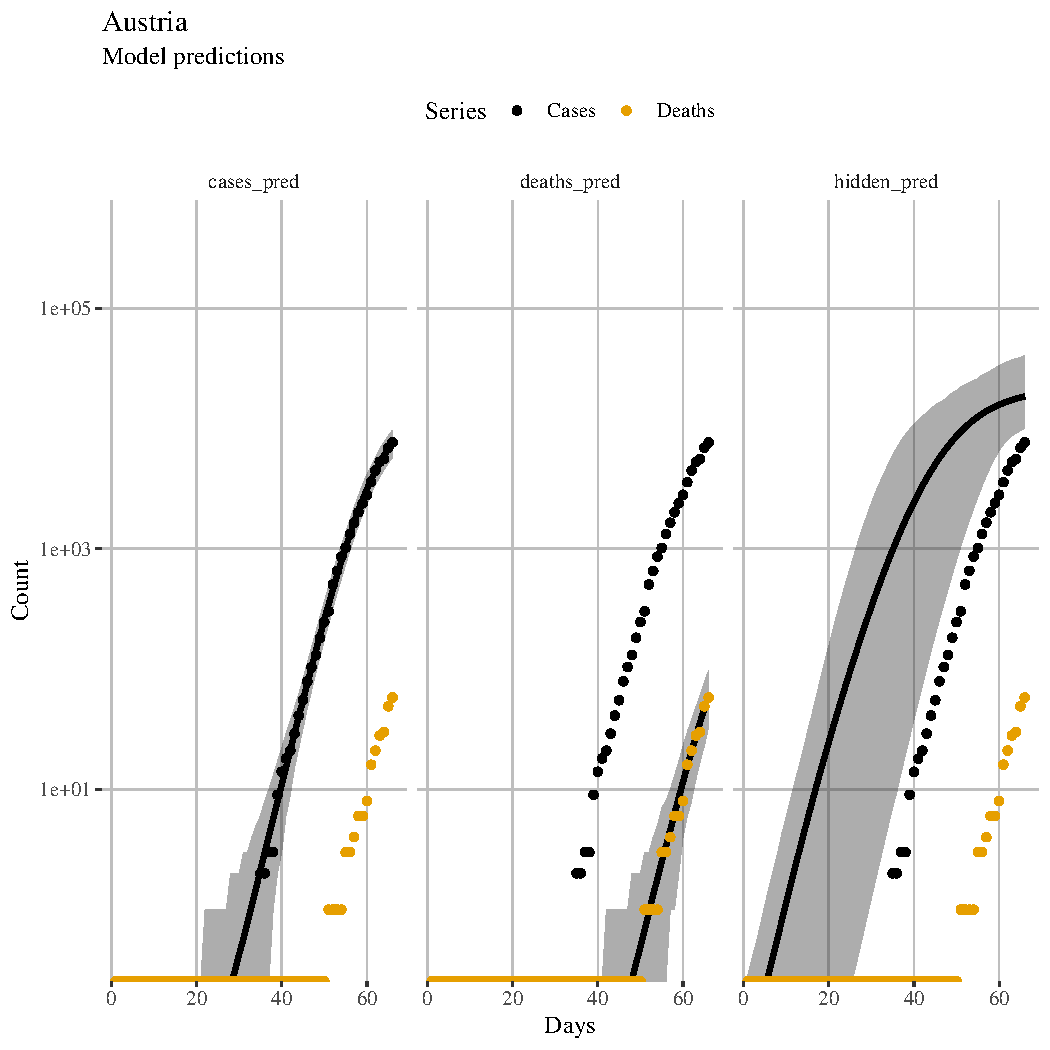
\includegraphics[width=0.45\textwidth]{../figs/model_pred_AUT.pdf}
    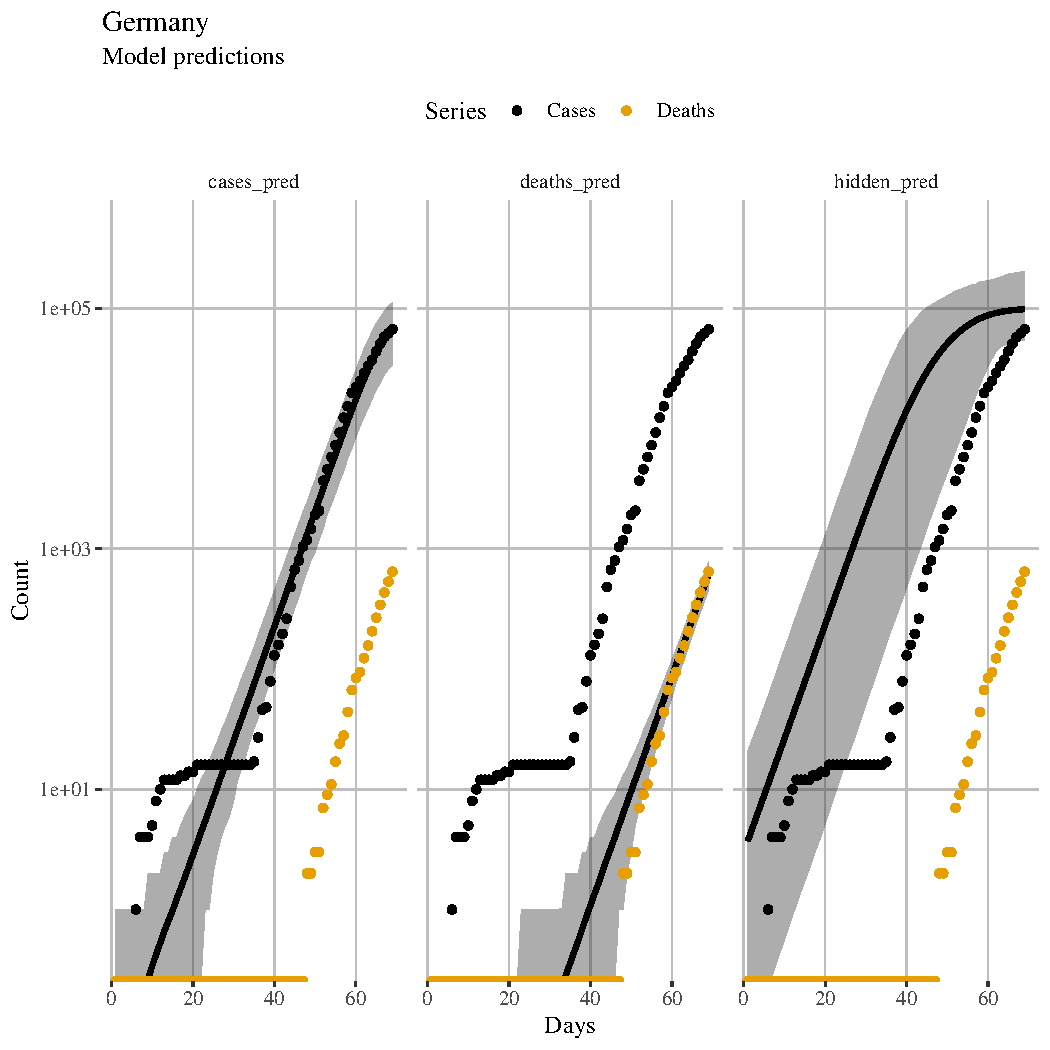
\includegraphics[width=0.45\textwidth]{../figs/model_pred_DEU.pdf}
    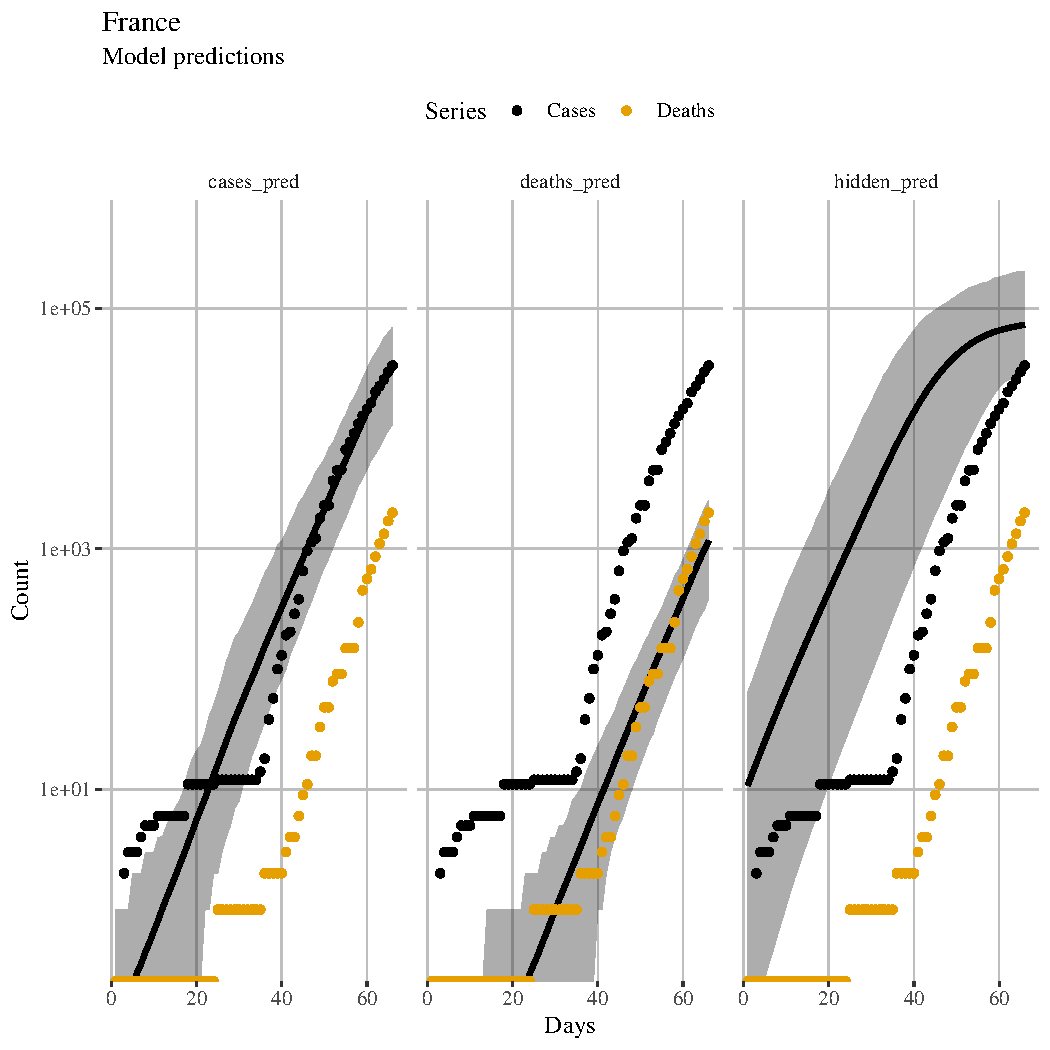
\includegraphics[width=0.45\textwidth]{../figs/model_pred_FRA.pdf}
    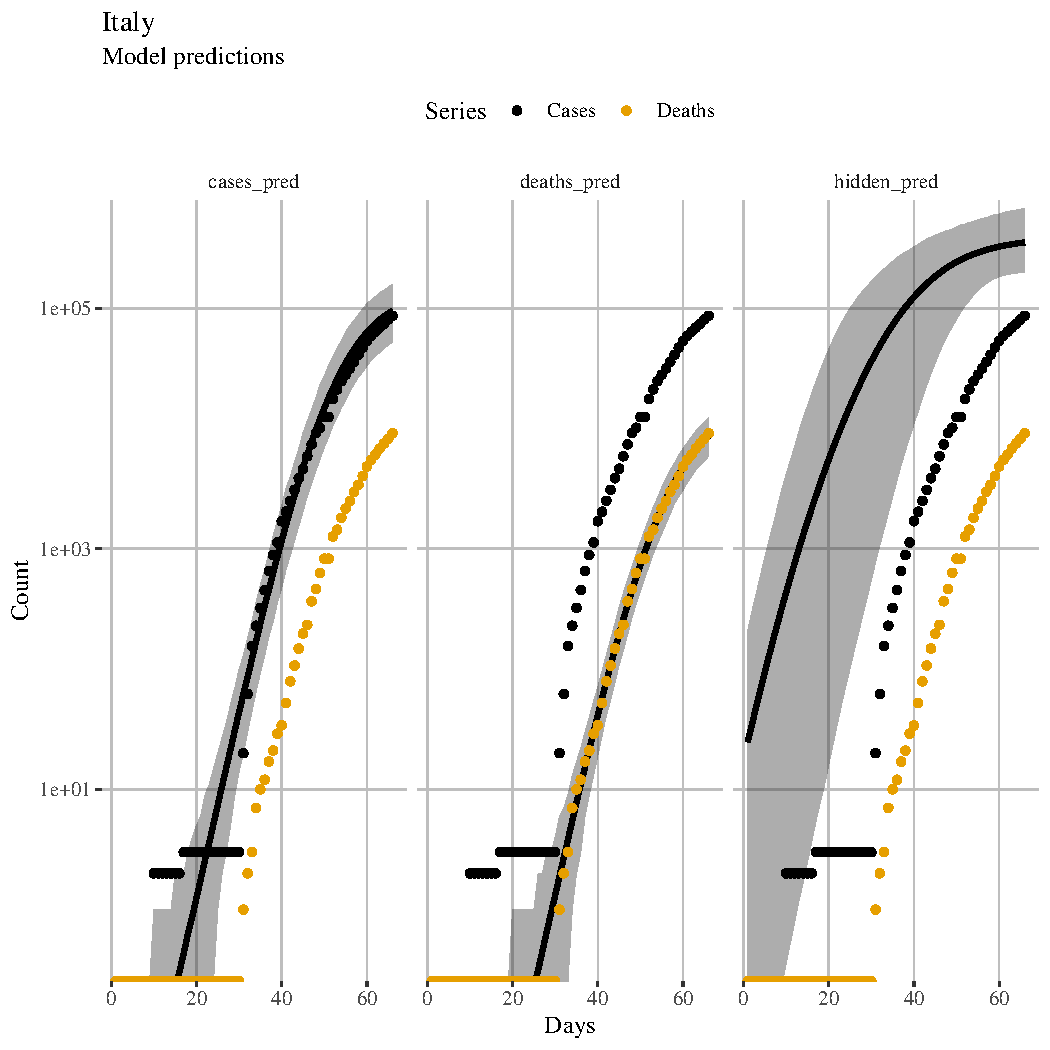
\includegraphics[width=0.45\textwidth]{../figs/model_pred_ITA.pdf}
    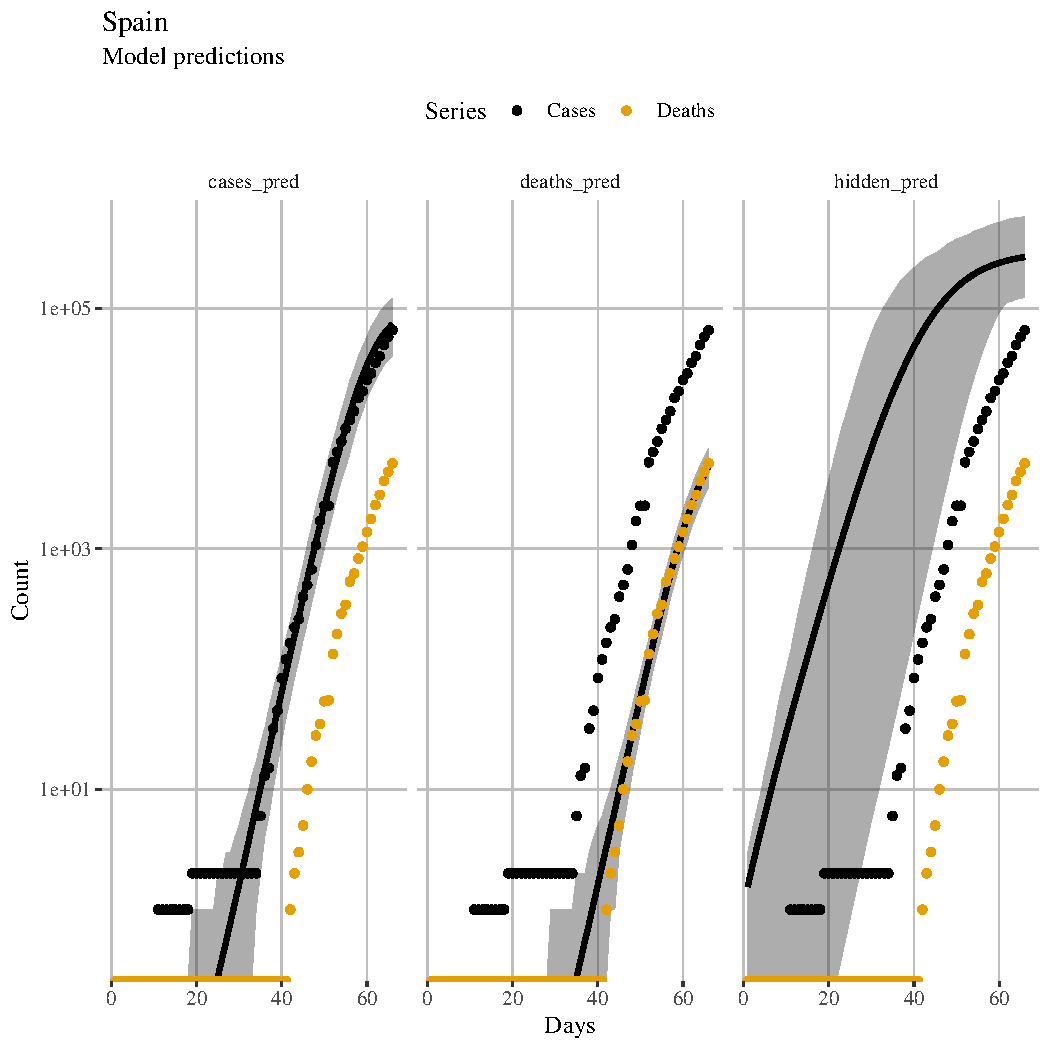
\includegraphics[width=0.45\textwidth]{../figs/model_pred_ESP.pdf}
    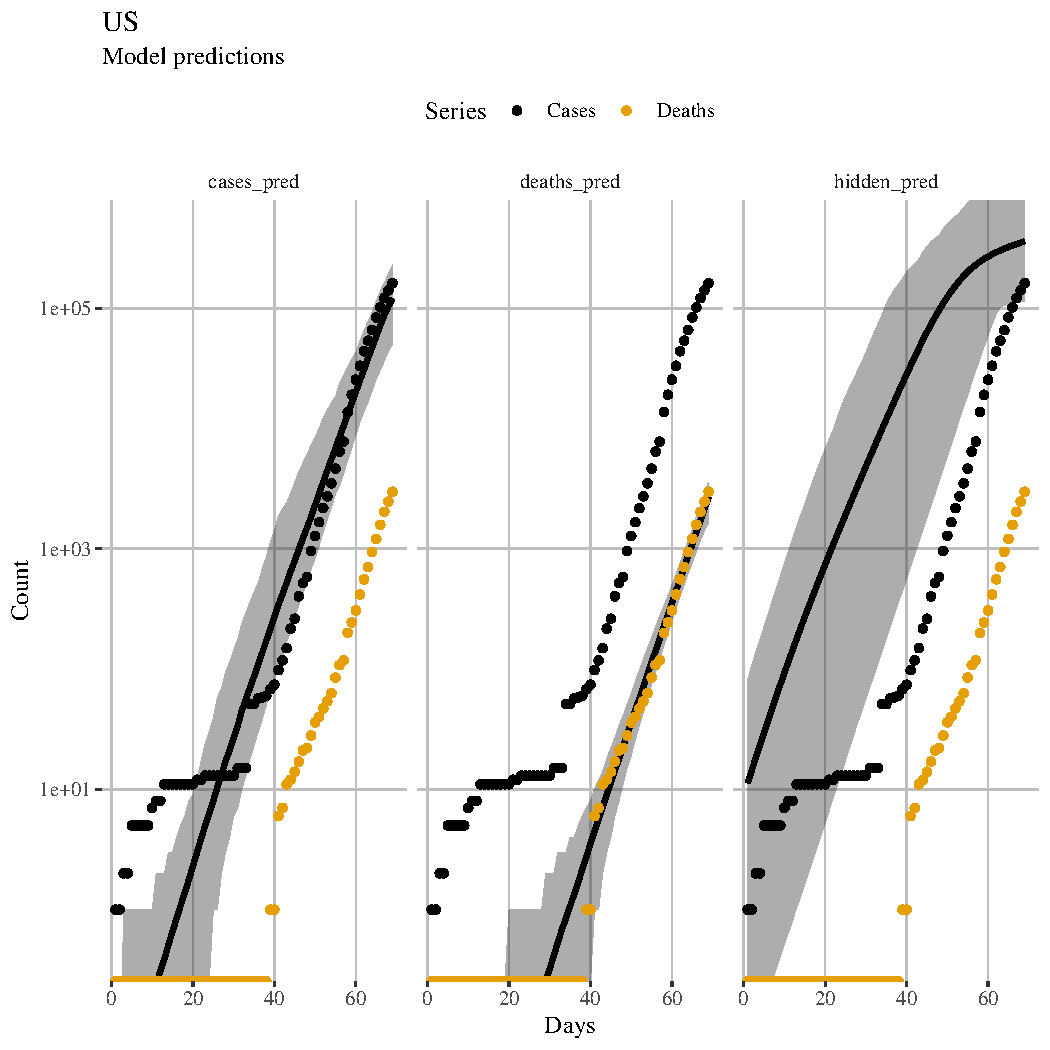
\includegraphics[width=0.45\textwidth]{../figs/model_pred_USA.pdf}
    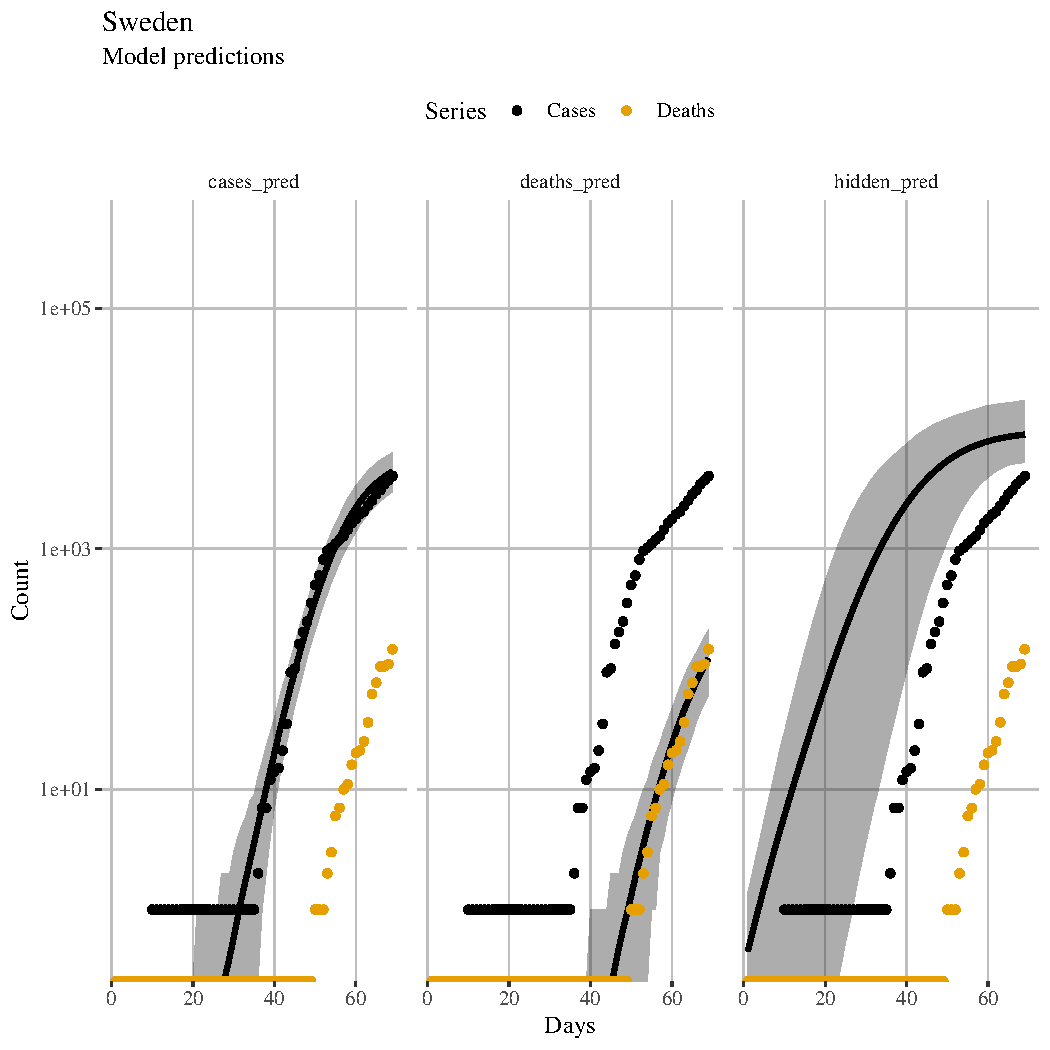
\includegraphics[width=0.45\textwidth]{../figs/model_pred_SWE.pdf}
    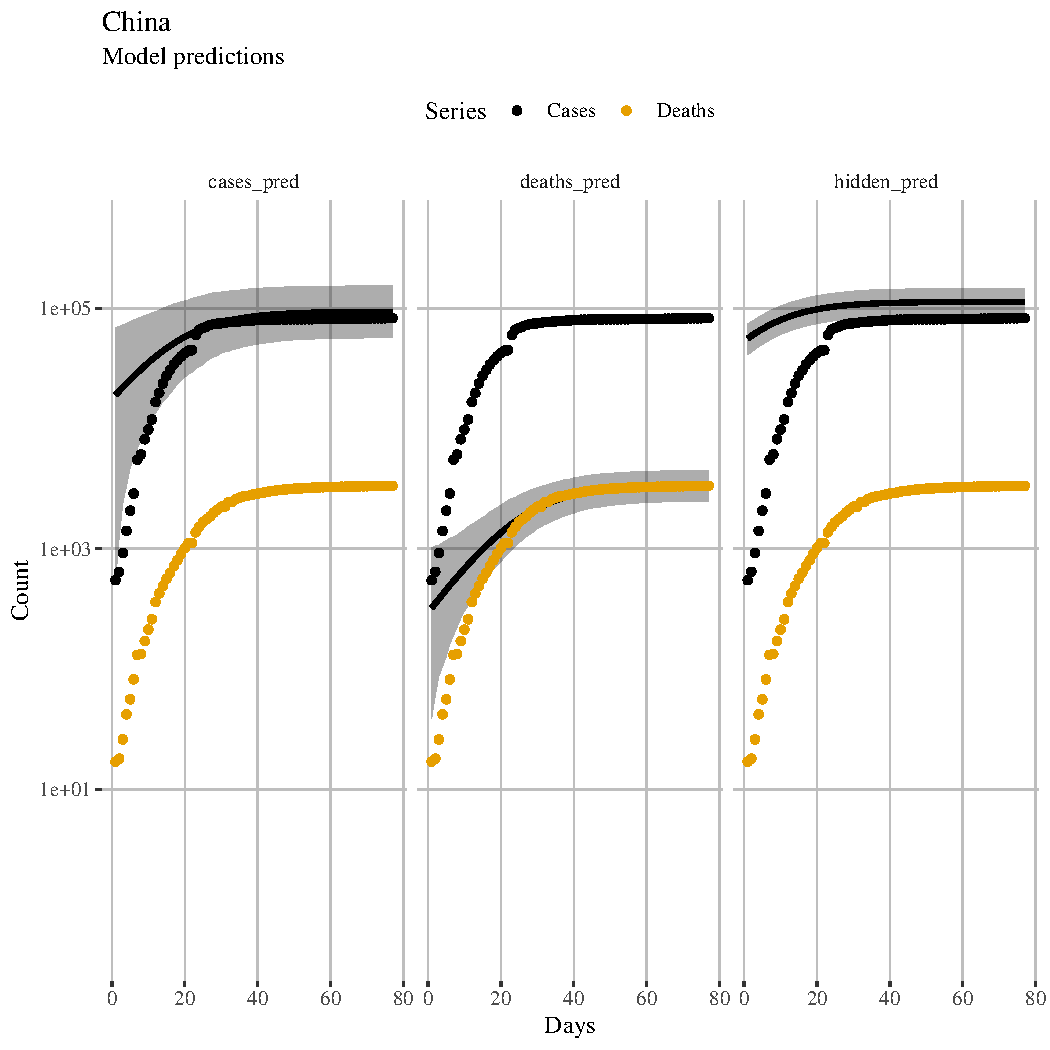
\includegraphics[width=0.45\textwidth]{../figs/model_pred_CHN.pdf}
    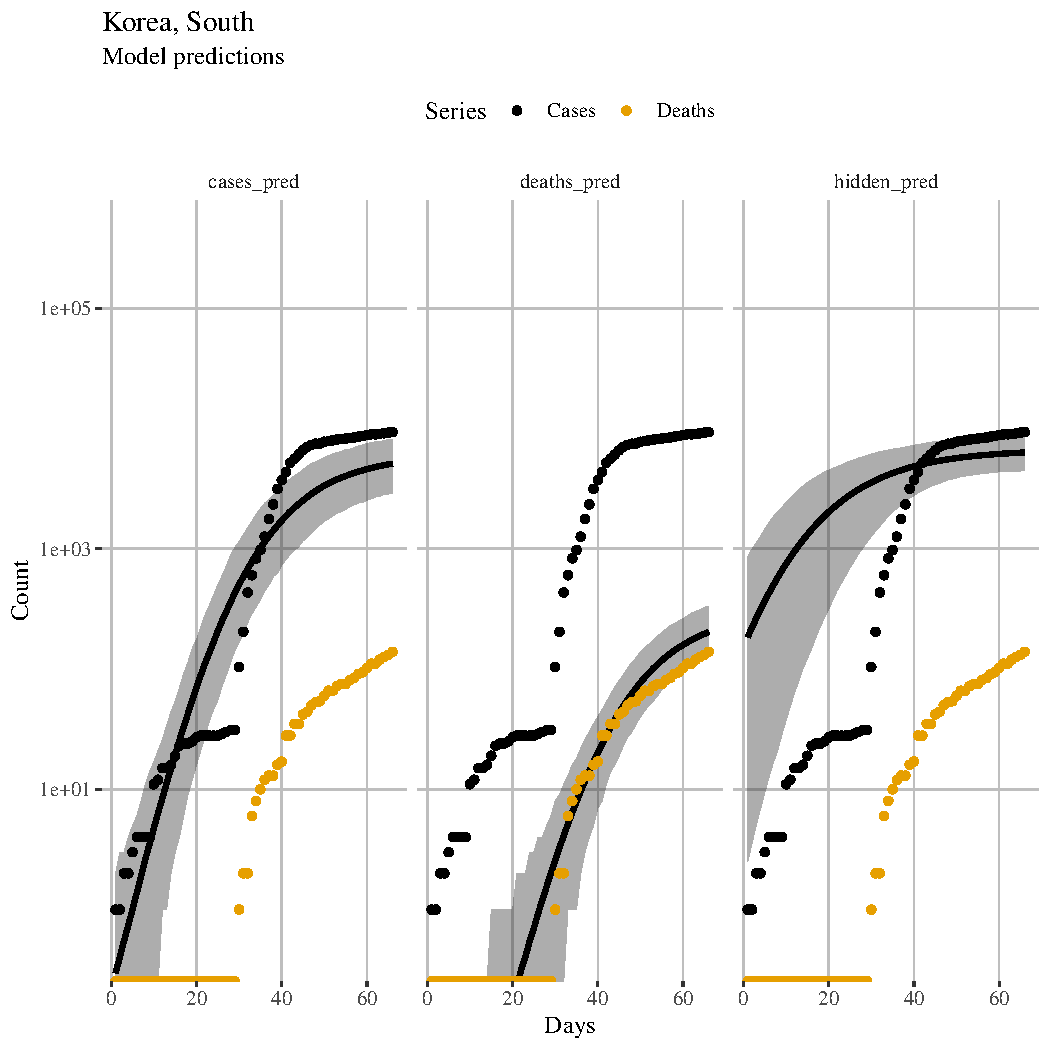
\includegraphics[width=0.45\textwidth]{../figs/model_pred_KOR.pdf}
    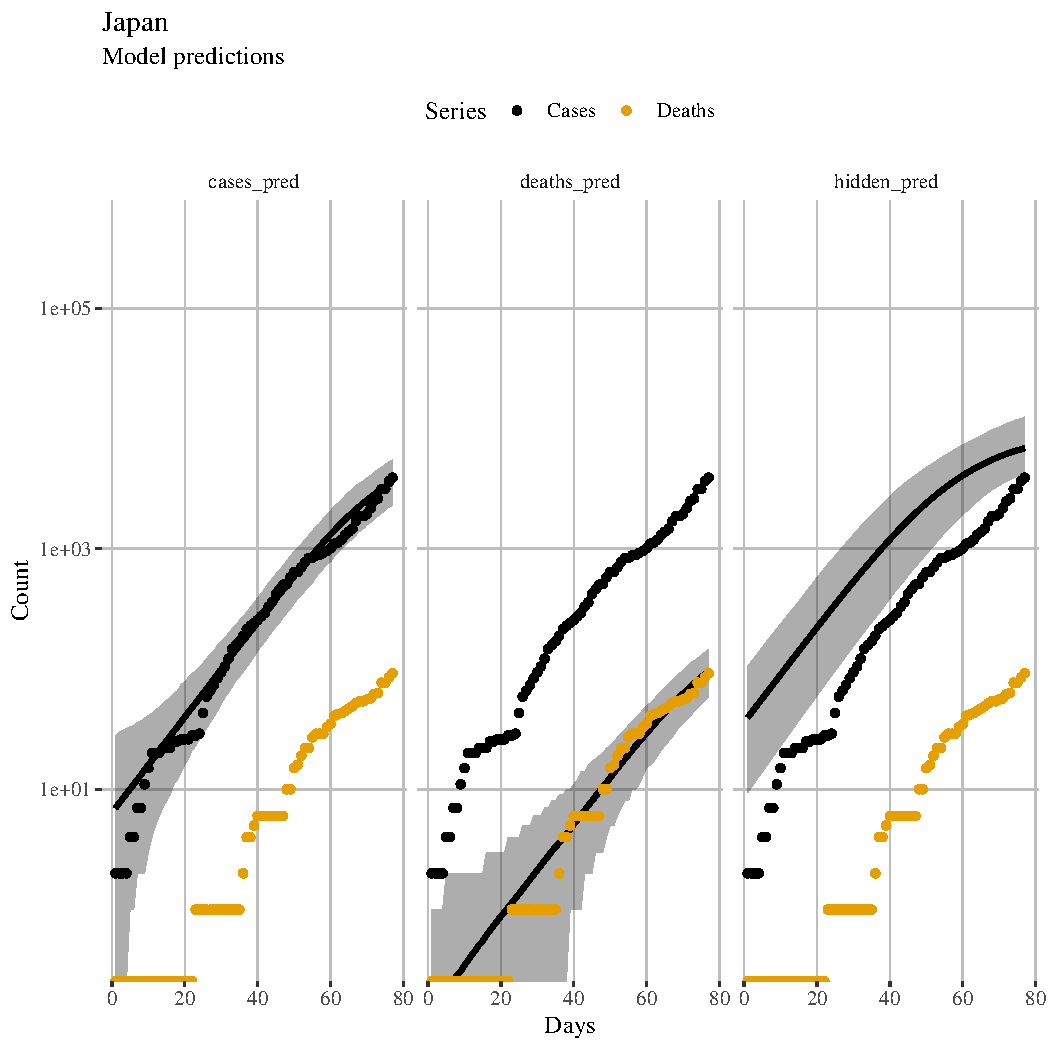
\includegraphics[width=0.45\textwidth]{../figs/model_pred_JPN.pdf}
  \end{center}
  \caption{\label{fig:modelpred} Model predictions (mean and 95\%
    credible region) of actual (hidden) and observed case and death
    counts for different countries. Note the log scale on the vertical
    axis.}
\end{figure}

\paragraph{Epidemic model}
The basic SIR model, assumes that an infection unfolds when
susceptible (S) individuals become infected (I) -- which in turn
infect further susceptible individuals. Finally, infected individuals
recover (R) (or die) and are no longer susceptible. In continuous
time, the dynamics can be described by the following system of
ordinary differential equations (ODEs):
\begin{align*}
  \frac{dS}{dt} &= - \beta \frac{I_t}{N} S_t \\
  \frac{dI}{dt} &= \beta \frac{I_t}{N} S_t - \gamma I_t \\
  \frac{dR}{dt} &= \gamma I_t
\end{align*}
where $N \equiv S_t + I_t + R_t$ is constant over time. Model
parameters are
\begin{itemize}
\item the infectivity $\beta$
\item and the recovery rate $\gamma$.
\end{itemize}
In this model, the average time of infection is $\gamma^{-1}$ giving
rise to a {\em base reproduction number} of $R_0 = \beta
\gamma^{-1}$.

\todo[inline]{Build and discuss model with delay effect \ldots}

\section{Financial markets}

Especially the containment measures implemented in many countries
around the world, have major economic consequences. Non-essential
productive activity has come to a hold and financial markets around
the world tanked. Furthermore, uncertainty is high and the volatility
index VIX has reached levels as during the financial crisis of 2007/8.
\begin{marginfigure}
  \begin{center}
    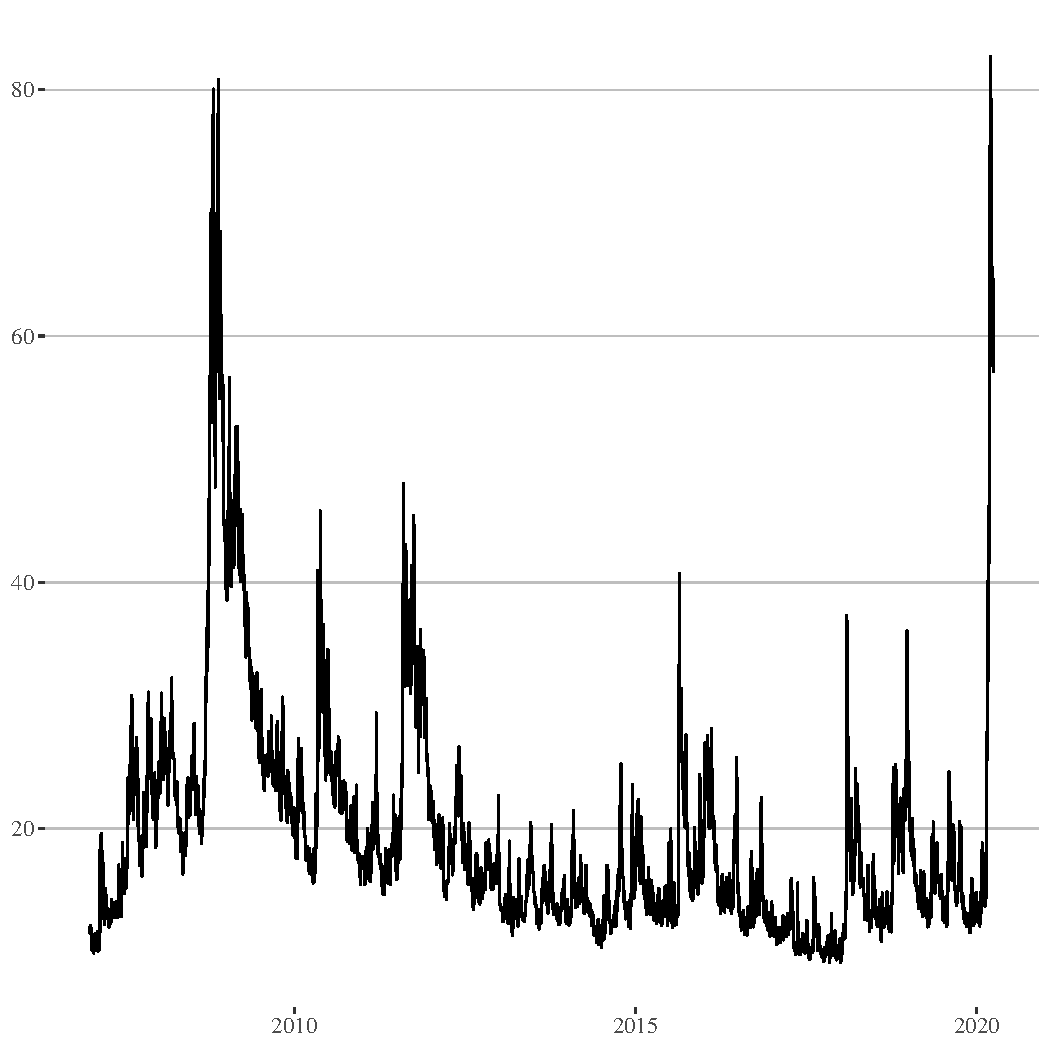
\includegraphics[width=0.95\textwidth]{../figs/VIX.pdf}
  \end{center}
  \caption{Closing values of VIX.}
\end{marginfigure}

\subsection{Implied risk-neutral densities}

To get an impression of the forward-looking market outlook, I
investigate call and put options on the S\&P 500 index. In particular,
out- or slightly in-the-money options are actively traded and also
utilized in the computation of the VIX. \fig{optionchain} shows the
corresponding prices of call and put options for different expiration
dates.
\begin{marginfigure}
  \begin{center}
    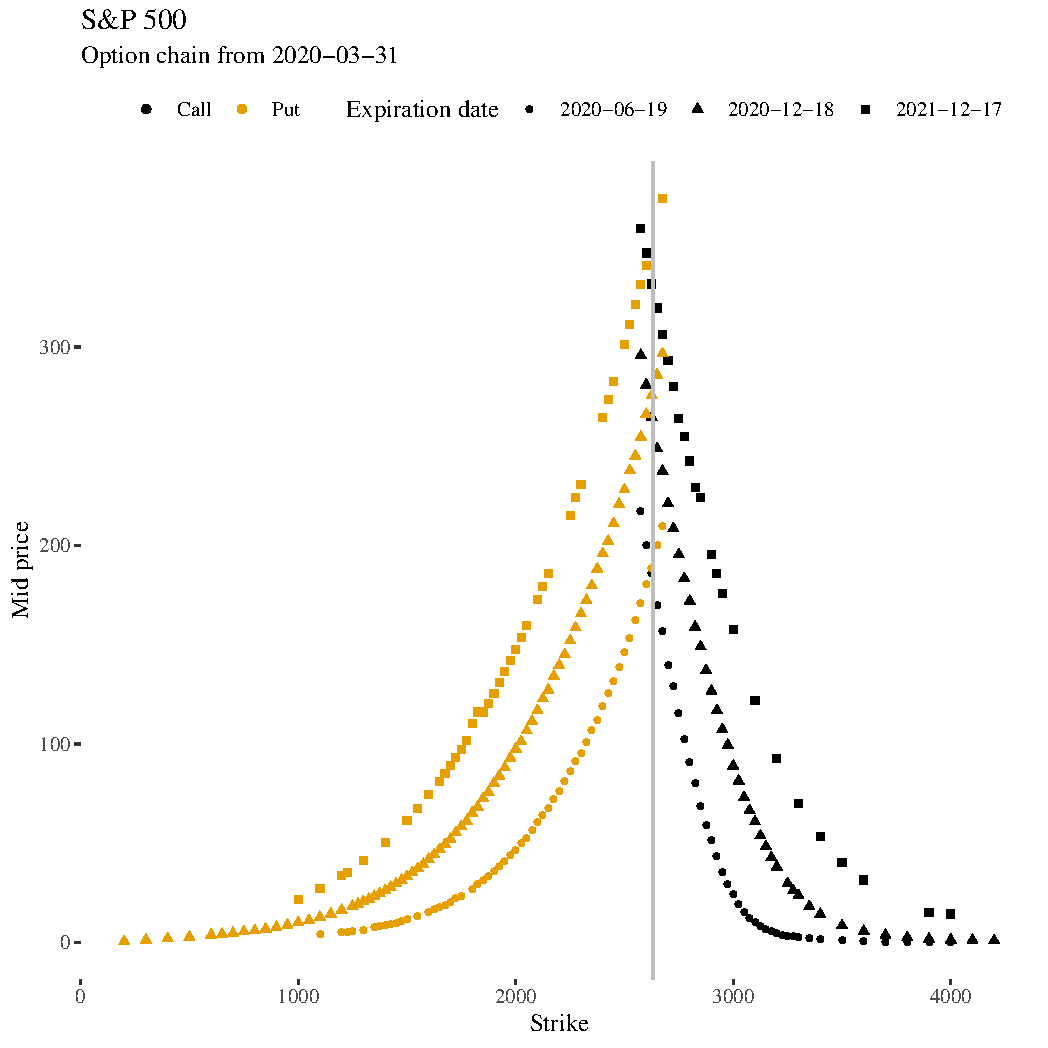
\includegraphics[width=0.95\textwidth]{../figs/option_chain.pdf}
  \end{center}
  \caption{\label{fig:optionchain} Mid prices of call and put options
    on the S\&P 500. Only out- or slightly in-the-money options with
    positive bid price are shown. The grey line marks the current spot
    price.}
\end{marginfigure}

By risk-neutral pricing, the current value of an option on the
underlying $S_t$ paying $v(S_T)$ at maturity $T$ is given as
\[ p_t = \E^{\Q}[e^{- r (T - t)} v(S_T)] \; , \]
where the expectation is taken over the risk-neutral measure $\Q$. In
particular, assuming a log-normal risk-neutral distribution $q(s_T)$
the well known Black-Scholes-Merton (BSM) formulas provides the
analytic price of European call and put options depending on the
risk-neutral interest rate $r$, maturity $T$, strike price $K$, spot
price $S_t$ and volatility $\sigma$. Unfortunately, the BSM has
several short-comings. Especially the assumption of constant
volatility does not hold in actual option prices giving rise to the
famous volatility-smile.

Nevertheless, the model is easily extended towards mixtures of
log-normal distributions. Then, by linearity of expectation values the
theoretical price is simply given as a weighted sum of BSM prices for
the different mixtures components. Here, we fit the above option
prices with a mixture of two components\footnote{Preliminary results
  show that more components only marginally improve the fit.}.
%% \begin{marginfigure}
%%   \begin{center}
%%     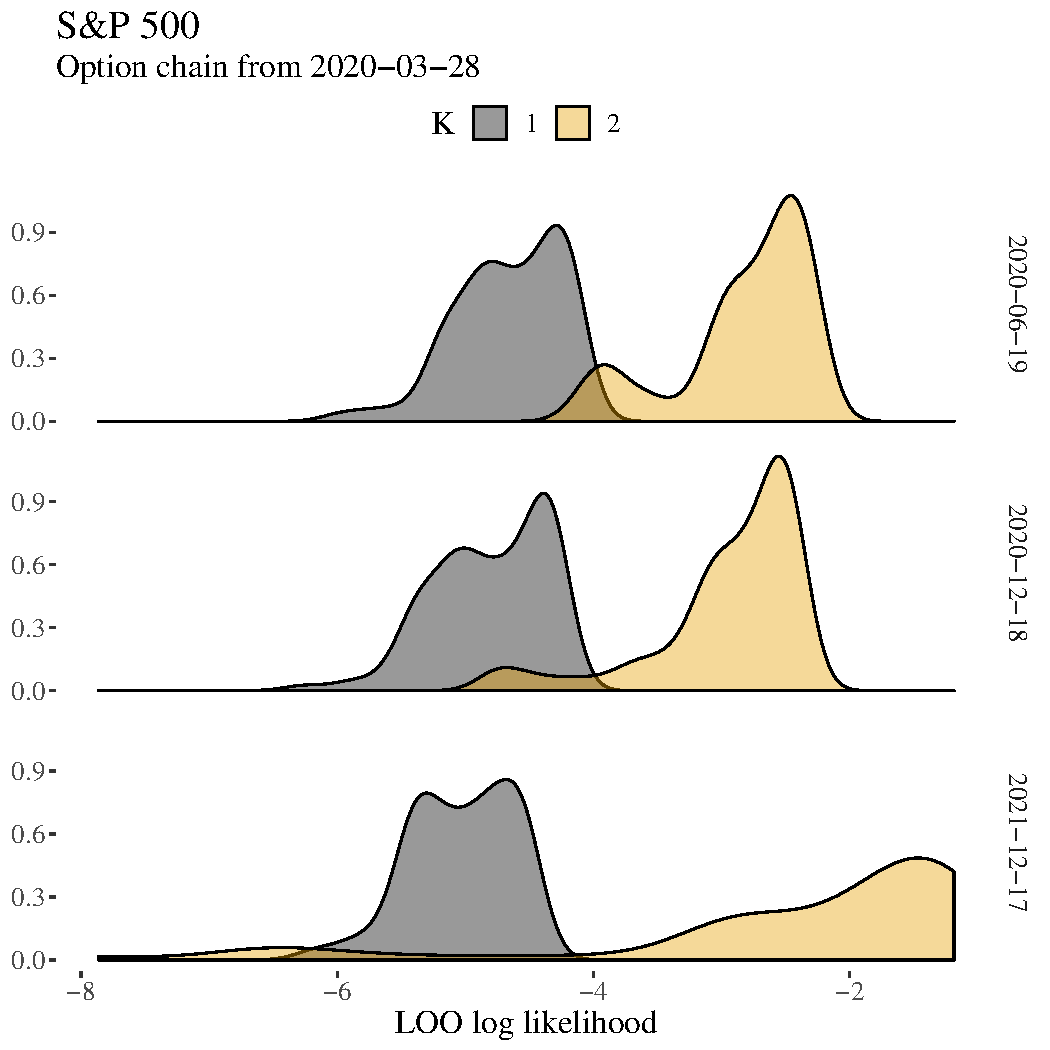
\includegraphics[width=0.95\textwidth]{../figs/model_loo.pdf}
%%   \end{center}
%%   \caption{Visual model comparison based on LOO log likelihood.}
%% \end{marginfigure}

Compared to a single component, the two component model is
substantially better and also nicely interpretable. In particular,
\fig{riskneutral} shows the implied components of the risk neutral
density. These can readily be interpreted as a good and bad market
outlook.
\begin{figure}
  \begin{center}
    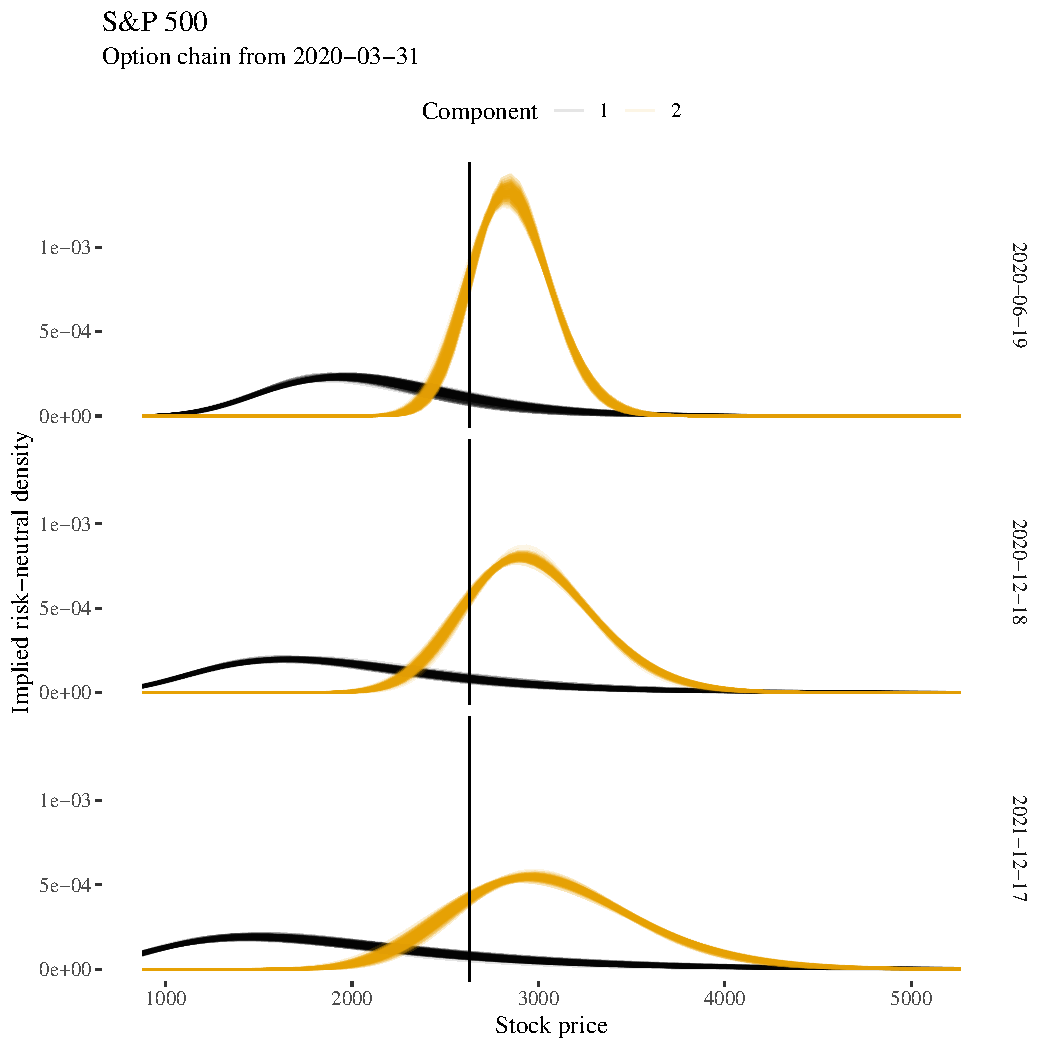
\includegraphics[width=0.95\textwidth]{../figs/risk_neutral.pdf}
  \end{center}
  \caption{\label{fig:riskneutral} Components of fitted implied
    risk-neutral density. Shown are 100 draws from the posterior
    distribution.}
\end{figure}
Indeed, \fig{crashprob} shows the implied crash probabilities,
i.e. weight assigned to the bad market component. These are
surprisingly high and even rise over longer maturities. In this sense,
option markets already price potentially long and large economic
distortions. Timely updates of this analysis will be provided and
hopefully the outlook will become more optimistic any time soon \ldots
\begin{marginfigure}
  \begin{center}
    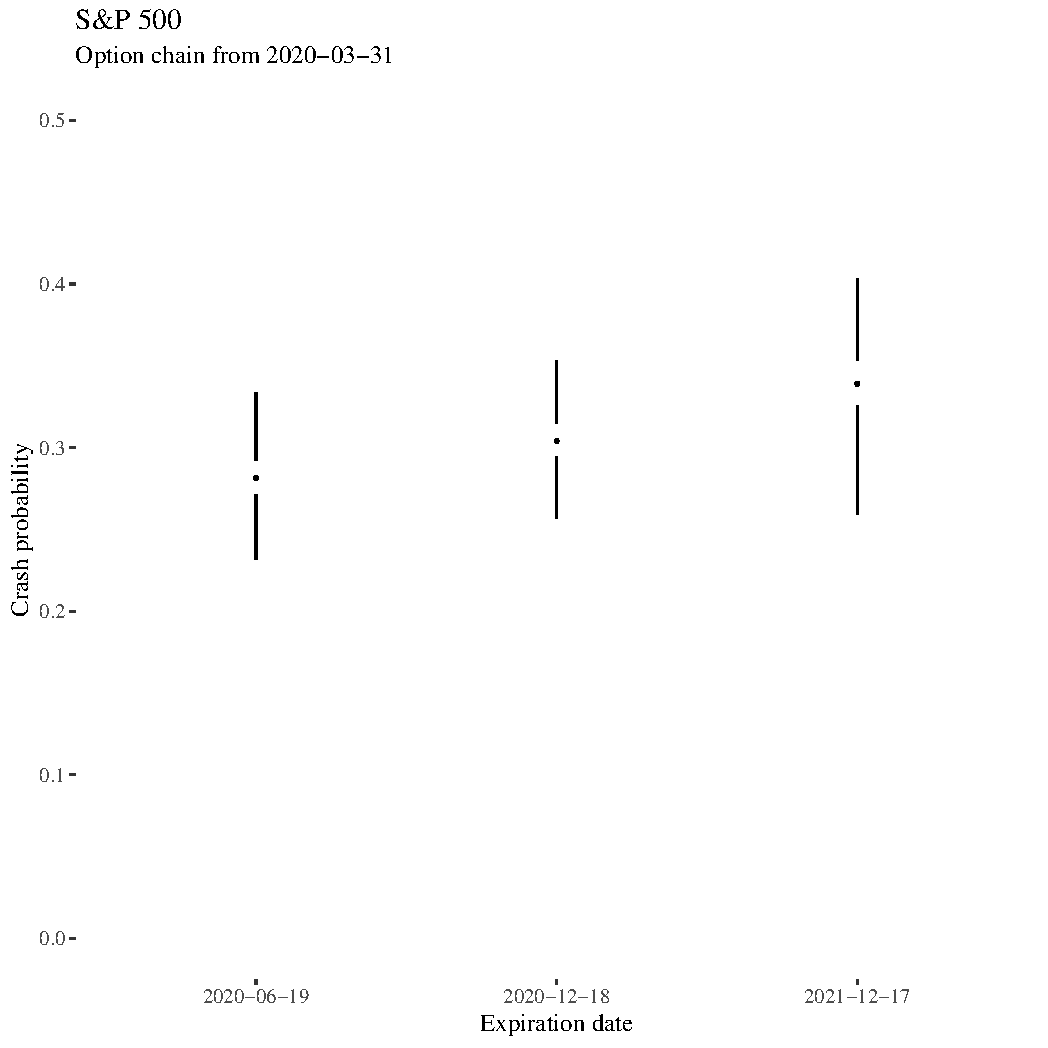
\includegraphics[width=0.95\textwidth]{../figs/crash_prob.pdf}
  \end{center}
  \caption{\label{fig:crashprob} Market implied crash probability
    derived from two component mixture model.}
\end{marginfigure}

\appendix

%% \section{Sigmoid model code}
%% \label{app:model}
%% \lstinputlisting[style=custom,firstline=1]{../../code/stan/growth.stan}

\end{document}
